\clearpage
\subsection{Box}  
\hypertarget{prettyboxplot}{}

\index{Plot Types!box}  
\index{Plot Types!box!basic}

 For box plots, you can use \texttt{pretty boxplot}.
\begin{figure}[h!]
	\begin{minipage}{0.7\textwidth}
		\begin{mintedtxtbox}[/data/box.tsv]
\begin{minted}{TeX}
%method1    ...        methodM
y1      y2      y3      y4
0.10    0.15    0.12    0.18 
... 
0.95    0.98    0.93    0.97
\end{minted}
		\end{mintedtxtbox}
\end{minipage}
\end{figure}
\begin{figure}[h!]
\begin{minipage}{0.65\textwidth} 
\begin{mintedtexbox}[/examples/box.tex]  
\inputminted{TeX}{lst/box.txt}
\end{mintedtexbox}  
	\end{minipage}
	\begin{minipage}{0.3\textwidth}  
		\def\file{data/box.tsv}
	\boxes{\file}[width=\textwidth]
\end{minipage}
\end{figure} 
  

Here is a different  look \cite{tufte2001visual}. 
\begin{figure}[h!]
	\begin{minipage}{0.65\textwidth} 
		\begin{tcolorbox}
			\begin{minted}{TeX} 
\begin{axis}[ pretty boxplot simple ]
\foreach \col in {y1,y2,y3,y4,y5,y6,y7,y8}{
    \addplot table[y=\col] {data/boxes.tsv};
}
\end{axis}
			\end{minted}
		\end{tcolorbox}
	\end{minipage}
\begin{minipage}{0.3\textwidth} 
\begin{tikzpicture}  
\begin{axis}[
pretty boxplot simple, width=\textwidth]
\foreach \col in {y1,y2,y3,y4,y5,y6,y7,y8}{
\addplot table[y=\col] {data/boxes.tsv};
}
\end{axis}
\end{tikzpicture}
 \end{minipage}  
 \end{figure} 
 \clearpage


\iffalse
\subsection{Violin Plot} 
\begin{figure}[h!]
	\begin{minipage}{0.65\textwidth}
		\begin{mintedtxtbox}[/data/box.tsv]
			\begin{minted}{TeX}
			\end{minted}
			%	\inputminted{TeX}{lst/box_data.txt}
		\end{mintedtxtbox}
	\end{minipage}
	\begin{minipage}{0.3\textwidth}	
		\begin{tikzpicture}
		\violinsetoptions[
		averages,
		data points,
		scaled,
		]{ pretty violin,
			xmin=0,xmax=5,
			ymin=0,ymax=3, 
			xlabel style={
				yshift = {-2*height("a")}
			}, 
			ylabel={Same property},
		}
		\violinplotwholefile[%
		primary color=blue, 
		secondary color=red, 
		indexes={A,B,C,D},
		spacing=1.0,
		labels={%
			$\alpha$,
			$\beta$,
			$\gamma$,
			$\delta$,
		},
		col sep=comma,
		dataset size=1pt,
		dataset mark=*,
		dataset fill=black!50!white,
		dataset fill opacity=1.0,
		average mark=diamond*,
		average size=5pt,
		]{data/violin.tsv}
		\end{tikzpicture}
	\end{minipage}
\end{figure}
\fi


\clearpage
\begin{comment} %todo fix some error here  
\subsection{Box (prepared)}
For large datasets, prepare the boxplots statistics (median, whiskers) in advance, as it takes long for pgfplots to compute them each time. For example, using \texttt{scripts/gen\_boxplot.py}. 
\begin{figure}[h!]
	\begin{minipage}{0.4\textwidth}
		\begin{tcolorbox}
			\begin{minted}{shell-session}
#run this to precompute boxplot statistics
#input: box-large.tsv (or .csv)
#outputs: box-large_stats.csv, box-large.tex 

> python gen_boxplot.py box-large.tsv
			\end{minted}
		\end{tcolorbox}
	\end{minipage}
\end{figure}
\begin{figure}[h!]
	\begin{minipage}{0.4\textwidth} 
		\begin{mintedtexbox}[/scripts/box-large.tex] 
			\begin{minted}{TeX}  
%% prepared version (15s)
%% using box-large_stats.tsv

\pgfplotstableread[col sep = comma]{scripts/box-large_stats.csv}\datatable
\begin{tikzpicture}
\begin{axis}[pretty boxplot, boxplot/draw direction=y, height=4cm]
\pgfplotstablegetrowsof{\datatable}
\pgfmathtruncatemacro\TotalRows{\pgfplotsretval-1}
\pgfplotsinvokeforeach{0,...,\TotalRows}
{
    \addplot+[
    boxplot prepared from table={
        table=\datatable,
        row=#1,
        lower whisker=lw,
        upper whisker=uw,
        lower quartile=lq,
        upper quartile=uq,
        median=med
    },
    boxplot prepared,
    ]
    coordinates {};

    %% comment out if column names should be legend entries: 
    %\pgfplotstablegetelem{#1}{name}\of\datatable
    %\addlegendentryexpanded{\pgfplotsretval}
}
\end{axis}
\end{tikzpicture}

			\end{minted}
		\end{mintedtexbox} 
		\begin{tcolorbox} 
			\begin{minted}{TeX}  
%% unprepared version 
%% using box-large.tsv
\boxes{scripts/box-large.csv}[][][col sep=comma]
			\end{minted}
		\end{tcolorbox}  
	\end{minipage}
	\begin{minipage}{0.6\textwidth} 
		
\pgfplotstableread[col sep = comma]{scripts/box-large_stats.csv}\datatable
\begin{tikzpicture}
\begin{axis}[pretty boxplot, boxplot/draw direction=y, height=4cm]
\pgfplotstablegetrowsof{\datatable}
\pgfmathtruncatemacro\TotalRows{\pgfplotsretval-1}
\pgfplotsinvokeforeach{0,...,\TotalRows}
{
    \addplot+[
    boxplot prepared from table={
        table=\datatable,
        row=#1,
        lower whisker=lw,
        upper whisker=uw,
        lower quartile=lq,
        upper quartile=uq,
        median=med
    },
    boxplot prepared,
    ]
    coordinates {};

    %% comment out if column names should be legend entries: 
    %\pgfplotstablegetelem{#1}{name}\of\datatable
    %\addlegendentryexpanded{\pgfplotsretval}
}
\end{axis}
\end{tikzpicture}
  
	%	\boxes{scripts/box-large.csv}[height=4cm][][col sep=comma]  
		\boxesFromStats{scripts/box-large_stats.csv}[height=4cm][][col sep=comma]  
	\end{minipage}
\end{figure} 
\end{comment}
\clearpage